\section{Muon + Hadronic Tau Channel}\label{sec:muTauhad}

The motivation for analyzing events where one $\tau$ lepton decays to a muon,
while the other decays to hadrons is the same for all \ditau related analyses: because
muons have the lowest jet misidentification among leptons, the mere requirement of a
muon removes a substantial amount of background processes, especially the QCD multijet background. Once this requirement
is made, a main source of background is due to Drell-Yan
processes giving rise to $\tau$ leptons. Because we seek particles with masses
much larger than that of the Z boson, this source of background can be easily discriminated
against by looking at larger reconstructed \ditau mass regions (reconstructed mass to be defined later). This process,
however, can also serve as a ``standard candle" to validate the $\tau_{h}$ identification criteria and
ensure the robustness of the analysis. Other main sources 
of background include (1) QCD multijet events where light-quark or gluon jets are misidentified 
as a $\tau_{h}$, (2) W + Jets events where the W boson decays to a muon and a jet is
misidentified as a $\tau_{h}$, and (3) $t\bar{t}$ events where two leptons can
come from the prompt decay of W bosons or one misidentified $\tau_{h}$ from a jet. The sum of the Drell-Yan and W + Jets backgrounds represent 
approximately $89$\% of the total background (according to simulation) in this channel.  The 
cuts used to select $\mu\tau_{h}$ pairs are factorized in to four categories: acceptance, 
$\mu$ identification, $\tau_{h}$ identification, and topological cuts. Acceptance criteria is completely
driven by the limitations of the CMS detector and the need to maximize analysis
sensitivity while also minimizing systematic effects. For example, in order to minimize systematic effects, the
$p_{T}$ threshold on the muon leg is chosen such that it falls on the plateau of the trigger turn-on curve ($p_{T} > 30$ GeV ... see Section \ref{sec:triggers}). 
Although it is possible to achieve slightly better sensitivity by increasing the thresholds,
the selections are also driven by the need to obtain a sample enriched with $Z\to\tau\tau$ events, 
with minimal modifications to the final selection criteria. 
Figure~\ref{fig:muTauKinematics} shows 
the $p_{T}$ distributions for signal and background processes relevant to this analysis. 
As discussed in section 5.3, the muon identification criteria is designed mostly to discriminate
against cosmic muons, punch-through pions, and muons associated to jets 
from decays in flight. The $\tau_{h}$ identification is described in section 5.4 and is mostly designed to
discriminate against hadronic jets produced from the fragmentation of quarks and/or
gluons. Finally, topological cuts are principally used to minimize the remaining W + jet(s)
and $t\bar{t}$ contributions after the muon and $\tau_{h}$ identification criteria have been
imposed. 

\begin{figure}\centering
  \includegraphics[width=0.4\textwidth]{figures/mt/Muon1Pt_ProbabilityPlot_AfterRecoTau1NmaxBeforeRecoBJetNmax.png}
  \includegraphics[width=0.4\textwidth]{figures/mt/TauJet1Pt_ProbabilityPlot_AfterRecoTau1NmaxBeforeRecoBJetNmax.png}
  \caption{\label{fig:muTauKinematics} Left: $p_{T}(\mu)$ after acceptance, $\mu$ identification, and $\tau_{h}$ identication cuts.  Right: 
$p_{T}(\tau_{h})$ after acceptance, $\mu$ identification, and $\tau_{h}$ identification cuts.}
\end{figure}

W boson production in association with jets becomes a dominant background because a clean, well-reconstructed muon is produced by the W boson. 
Therefore, the requirement of a clean muon signature does not provide additional discrimination. Additionally, the neutrino from the W boson decay acquires 
an average energy of approximately $m_{W}/2 \sim 40$ GeV. Because the neutrino will escape the CMS detector undetected, the average measurement of the momentum 
imbalance will be approximately 40 GeV. Therefore, our requirement on the momentum imbalance in the event ($\MET > 30$ GeV) does not provide significant 
discrimination against this background. 
Figure~\ref{fig:muTauTopologicalVariables} shows
the $\MET$ distribution for signal and background processes relevant to this analysis. 
Finally, the presence of ``associated jets" means that the contamination from W + Jets in the signal region is 
highly dependent on the jet$\to\tau_{h}$ fake rate, which is the largest among leptons. Therefore, reducing W + Jets also requires additional 
topological requirements. 

\begin{figure}\centering
  \includegraphics[width=0.4\textwidth]{figures/mt/Met_ProbabilityPlot_AfterRecoBJetNmaxBeforeSusyCombinationsNmin.png}
  \includegraphics[width=0.4\textwidth]{figures/mt/Muon1Tau1Zeta1D_ProbabilityPlot_AfterRecoBJetNmaxBeforeSusyCombinationsNmin.png}
  \caption{\label{fig:muTauTopologicalVariables} Left: $\MET$ after acceptance, $\mu$ identification, and 
$\tau_{h}$ identication cuts.  Right: $P_{\zeta}- 3.1 \times P_{\zeta}^{vis}$ after acceptance, $\mu$ identification, and $\tau_{h}$ identication cuts.}
\end{figure}

In W + jet(s) events, unlike $X\rightarrow\tau\tau$ resonance production such as $Z^{\prime} \to \tau\tau$, where the $\tau$-lepton decay products are expected to 
be back-to-back in $\phi$, the presence of the neutrino from the $W$ decay and the uncorrelated jet gives rise to topologies where the jet and the lepton are not 
back-to-back (Figure~\ref{fig:WjetsRejectionDelPhiFigure}). Therefore, one of the main 
discriminating variables against W + Jets events is the difference in $\phi$ between the jet and muon directions. 
Figure~\ref{fig:MuTauMass} shows the cos$\Delta \phi(\mu,\tau_{h}/jet)$ distributions for $Z^\prime\to\tau\tau$ and the relevant background samples. 
We require 
\begin{equation}
\cos\Delta\phi(\mu,\tau_{h}/jet) < -0.95
\end{equation}
\noindent which is approximately $> 90$\% efficient for $Z^{\prime} \to \tau\tau$ and approximately 25\% efficient for W+Jets.

\begin{figure}
\begin{center}
\includegraphics[angle=0,width=.5\textwidth]{figures/mt/WjetsRejectionDelPhiFigure.pdf}
\caption{ Sketch depicting the W+Jets rejection power of a $\Delta \phi$ cut.}
\label{fig:WjetsRejectionDelPhiFigure}
\end{center}
\end{figure}
%\begin{figure}
%\begin{center}
%\includegraphics[angle=0,width=.5\textwidth]{figures/mt/Muon1Tau1CosDphi_ProbabilityPlot_AfterRecoBJetNmaxBeforeSusyCombinationsNmin.png}
%\caption{ cos$\Delta \phi$ between the muon and tau/jet directions.}
%\label{fig:MuonTauCosDelPhi}
%\end{center}
%\end{figure}\\

For \ditau final states, the $\MET$ in the event is due to the neutrinos from the $\tau$-lepton decays and is expected to point in the direction collinear 
to the visible tau decay products. Furthermore, the measurement of $\MET$ is completely correlated to the visible tau decay products. In W + jet(s) 
events, the direction and magnitude of the momentum imbalance is completely correlated to the lepton from the $W$ boson, but 
uncorrelated to the jet. We require events to be consistent with this signature of a particle decaying to two $\tau$ leptons by defining a unit vector along the 
bisector of visible tau decay products ($\hat{\zeta}$) and two projection variables, $p_{\zeta}$ and $p_{\zeta}^{vis}$:

\begin{equation}
   p_{\zeta}^{vis} = \overrightarrow{p}_{\tau_{1}}^{vis}\hat{\zeta}+\overrightarrow{p}_{\tau_{2}}^{vis}\hat{\zeta}
\label{eq:zetavis}
\end{equation}
\begin{equation}
   p_{\zeta} = p_{\zeta}^{vis}+\overrightarrow{{E\!\!\!\!/_{\rm T}}}\hat{\zeta}
\label{eq:zeta}
\end{equation}

The sketch in Figure~\ref{fig:ZetaDiagram} displays the definitions for $p_{\zeta}^{vis}$ and $p_{\zeta}$. Figures~\ref{fig:WjetsZeta1} and~\ref{fig:WjetsZeta2} 
show the separation between $Z^{\prime}\rightarrow\tau\tau$ and W + jet(s) events in the $p_{\zeta}$-$p_{\zeta}^{vis}$ plane. For the case of W+Jets, there is no 
strong correlation between $p_{\zeta}^{vis}$ and $p_{\zeta}$ due to the presence of a jet that is uncorrelated to the $\mu$ and $\nu_{\mu}$ from the W boson. 
However, there is a strong correlation for the case of $Z^{\prime} \to \tau\tau$. To discriminate against W+jet(s) events, requirements on $\Delta \phi 
(\tau_{1},\tau_{2})$ and $\zeta$ are applied. $\zeta$ is defined as a linear combination of $p_{\zeta}$ and $p_{\zeta}^{vis}$:

\begin{itemize}
  \item $cos\Delta\phi(\tau_{1},\tau_{2}) < -0.95$
  \item $p_{\zeta} - 3.1 p_{\zeta}^{vis} > -50$
\end{itemize}
\begin{figure}
\begin{center}
\includegraphics[angle=0,width=.75\textwidth]{figures/mt/zeta.png}
\caption{ Definitions for $p_{\zeta}$ and $p_{\zeta}^{vis}$.}
\label{fig:ZetaDiagram}
\end{center}
\end{figure}
\begin{figure}
\begin{center}
\includegraphics[angle=0,width=.5\textwidth]{figures/mt/Zeat2D_Ztautau.pdf}
\caption{ $p_{\zeta}$ vs. $p_{\zeta}^{vis}$ for $Z^{\prime}\rightarrow\tau\tau$.}
\label{fig:WjetsZeta1}
\end{center}
\end{figure}
\begin{figure}
\begin{center}
\includegraphics[angle=0,width=.5\textwidth]{figures/mt/Zeta2D.pdf}
\caption{ $p_{\zeta}$ vs. $p_{\zeta}^{vis}$ for W+Jets.}
\label{fig:WjetsZeta2}
\end{center}
\end{figure}

Although events containing $t\overline{t}$ contribute to the expected background in all channels containing light leptons, it's contribution to the $\mu\tau_{h}$ 
channel is only $\sim 1.4$\% of the total background (according to simulation). For $\mu\tau_{h}$ final states the 
$t\overline{t}$ contribution comes in the form of a real light lepton from the semileptonic decay of the
$W^\pm$ and a fake $\tau_{h}$ from the hadronic decay of the second $W^\pm$. These events are characterized by an isolated light lepton, passing all lepton 
identification and isolation requirements, accompanied by a non--isolated ``hadronic tau" due to the
larger multiplicity of the hadronically decaying W boson. 
%The case where the second $W^\pm$ decays semileptonically into a tau results in an event containing 
%isolated light leptons and taus that satisfy all identification and isolation requirements. 
These events are suppressed with the use of topological cuts.

After only applying lepton identification and isolation requirements, a non-negligible background contribution from $t\overline{t}$ events remain. These events 
can be further suppressed with cuts that take advantage of the very different topologies between $Z^\prime\to\tau\tau$ and $t\overline{t}$ events. The first, and most 
important, of these differences is the presence of b--jets in the event. 
%Other important differences include the presence of extra jets and the angle between the 
%${E\!\!\!\!/_{\rm T}}$ object and the highest 
%$p_{T}$ lepton in the event.\\
%The first tool to identify and reject $t\overline{t}$ events is counting the number of jets in the event are tagged as b--jets.  
For our purposes, jets with 
$p_{T} > 30$ GeV/$c$ and $|\eta| < 2.4$ are counted as b--tagged jets if the ``combined secondary vertex" discriminator, described in section 5, 
returns a value consistent with that of a b--jet. 
%The  ``track counting" discriminators are very simple, yet robust discriminators that return the significance of 
%the second  (hiEff) or third (hiPurity) most significant track  in the jet. 
In this analysis, the ``loose" operating point of the ``combined secondary vertex" 
discriminator (CSVL) is used. 
%The TCHEM discriminator requires a discriminant larger than 3.3 $\sigma$ for a jet to be tagged as a b--jet. The 
%mis-tag rate  associated with the ``medium" operating point is 1\% \cite{BjetCommissioning}. Figure~\ref{fig:JetTCHE} shows the TCHE b-jet discriminator for jets 
%in $Z^{\prime} \to \tau \tau$ and various backgrounds. Jets considered for b-tagging are required to be well separated from the tagged $\mu\tau_{h}$ pair 
%($\Delta 
%R(jet,\mu / \tau_{h})>0.5$).\\

The entire signal selection criteria are summarized below, while Table~\ref{tab:muTauCutFlowEff} is the cut flow efficiency table (yields normalized to $\sigma 
\cdot L \cdot \varepsilon$).

\textbf{Acceptance Selection:}

\begin{itemize}
  \item Events must fire the HLT{\_}IsoMu18 trigger
  \item $\ge 1$ global $\mu$ with $|\eta| < 2.1, p_{T} > 30$ GeV
  \item $\ge 1$ HPS $\tau_{h}$ with $|\eta| < 2.1, p_{T} > 20$ GeV
  \item $\Delta R(\mu,\tau_{h}) > 0.5$
\end{itemize}

\textbf{$\mu$ Identification:}

\begin{itemize}
  \item ``isMediumMuon"
  \item Relative isolation (with $\delta\beta$ corrections) $< 0.15$
\end{itemize}

\textbf{$\tau_{h}$ Identification:}

\begin{itemize}
  \item Muon veto: ``againstMuonTight3"
  \item Electron veto: ``againstElectronMVAVLooseMVA5"
  \item ``new" decay mode finding with 1 or 3 signal charged hadrons
  \item Isolation: ``byTightCombinedIsolationDeltaBetaCorr3Hits"
\end{itemize}

\textbf{Topological requirements:}

\begin{itemize}
  \item $\cos \Delta \phi (\mu,\tau_{h})$ $<$ -0.95. The $\tau_{h}$ jet direction is calculated using the sum of the four-momenta of decay mode constituents:
\begin{equation}
   \overrightarrow{p}_{\tau_{h}} = \sum_{i} \overrightarrow{p}_{signal\mbox{ }constituents}^{i}
   \label{eq:taudirection}
\end{equation}
  \item $Q(\mu) \times Q(\tau_{h}) < 0 $
  \item $\MET$ $>$ 30 GeV
  \item $P_{\zeta}- 3.1 \times P_{\zeta}^{vis} > -50$
  \item 0 jets tagged as b-jets
\end{itemize}

Because $\tau$ leptons decay to neutrinos which leave the detector undetected, one cannot fully reconstruct the mass resonance with the visible $\tau$ decay 
products. Additionally, because the invariant mass for background processes such as QCD are typically steeply falling distributions in the tails (where new mass 
resonances are expected), it becomes important to make use of $\MET$ to attempt to separate signal from background and reconstruct the true mass 
resonance. Historically, several methods such as the collinear approximation have been employed to reconstruct the true mass resonance. However, for the analysis 
presented, one of the main sources of backgrounds is W + jet(s). In this case, the analysis achieves a high degree of sensitivity by requiring the 
$\mu$ and $\tau_{h}$ candidates to be back-to-back in $\phi$ (see above description). This is precisely the regime in 
which the collinear approximation fails. Therefore, the mass is reconstructed as follows:

\begin{equation}
   M(\tau_{1},\tau_{2},{E\!\!\!\!/_{\rm T}}) = \sqrt{(E_{\tau_{1}}+E_{\tau_{2}}+{E\!\!\!\!/_{\rm
T}})^{2}-(\overrightarrow{p_{\tau_{1}}}+\overrightarrow{p_{\tau_{2}}}+\overrightarrow{{E\!\!\!\!/_{\rm T}}})^{2}}
\label{eq:ditaumass}
\end{equation}

\noindent where $E_{\tau}$ and $\overrightarrow{p_{\tau}}$ represent the energy and 4-momentum of the visible objects (in this case the $\mu$ and $\tau_{h}$), respectively.  As can be seen from Figure~\ref{fig:MuTauMass}, this definition successfully distinguishes 
between lower mass production of $\tau$-lepton pairs and high-mass $\tau$-lepton pairs from new massive resonant particle production.

\begin{figure}\centering
  \includegraphics[angle=0,width=.4\textwidth]{figures/mt/Muon1Tau1CosDphi_ProbabilityPlot_AfterRecoBJetNmaxBeforeSusyCombinationsNmin.png}
  \includegraphics[angle=0,width=.4\textwidth]{figures/mt/Muon1Tau1ReconstructableMass_ProbabilityPlot_AfterRecoBJetNmaxBeforeSusyCombinationsNmin.png}
  \caption{\label{fig:MuTauMass} Left: cos$\Delta \phi$ between the muon and tau/jet directions.  Right: $m(\mu,\tau_{h},\MET)$ for signal $Z^{\prime}$ 
and various backgrounds.}
\end{figure}
%\begin{figure}
%\begin{center}
%\includegraphics[angle=0,width=.75\textwidth]{figures/mt/Muon1Tau1ReconstructableMass_ProbabilityPlot_AfterRecoBJetNmaxBeforeSusyCombinationsNmin.png}
%\caption{ $m(\mu,\tau_{h},\MET)$ for signal $Z^{\prime}$ and various backgrounds.}
%\label{fig:MuTauMass}
%\end{center}
%\end{figure}


\begin{table}[htbp!]
\begin{center}
  \caption{Event summary table after signal region selection\label{tab:summaryTableMuTau}}
  \begin{tabular}{| l | c | c | c | c |}
  \hline
       Process          & \ditauh             & \mutau                 & \etau                 & \emu            \\ \hline
       $Z^\prime$ (500)         & 307.4 $\pm$ 35.3  & 502.3 $\pm$ 57.7      & 197.6 $\pm$ 22.7      & 218.6 $\pm$ 27.3  \\   
       $Z^\prime$ (1000)        & 34.6 $\pm$ 2.6    & 40.8 $\pm$ 3.1        & 14.7 $\pm$ 1.1        & 19.0 $\pm$ 1.5        \\   
       $Z^\prime$ (1500)        & 6.6 $\pm$ 0.3     & 7.2 $\pm$ 0.3         & 2.3 $\pm$ 0.1         & 3.6 $\pm$ 0.2      \\   
       $Z^\prime$ (2000)        & 1.6 $\pm$ 0.07    & 1.8 $\pm$ 0.08        & 0.59 $\pm$ 0.03       & 0.91 $\pm$ 0.04        \\   
       $Z^\prime$ (2500)        & 0.55 $\pm$ 0.02   & 0.60 $\pm$ 0.02       & 0.19 $\pm$ 0.01       & 0.30 $\pm$ 0.01       \\   
       $Z^\prime$ (3000)        & 0.13 $\pm$ 0.01   & 0.14 $\pm$ 0.01       & 0.04 $\pm$ 0.00       & 0.07 $\pm$ 0.00   \\   
       Drell-Yan        & 8.4 $\pm$ 3.1     & 882.4 $\pm$ 127.0     & 375.1 $\pm$ 117.6     & 321.2 $\pm$ 99.2 \\
       W+Jets           & 0.1 $\pm$ 0.1     & 916.2 $\pm$ 96.1      & 545.8 $\pm$ 85.6      & 18.9 $\pm$ 11.4 \\
       Diboson          & 0.5 $\pm$ 0.5     & 29.2 $\pm$ 7.4        & 18.0 $\pm$ 4.4        & 108.3 $\pm$ 17.4 \\
       $t\bar{t}$       & --                & 26.1 $\pm$ 6.7        & 26.1 $\pm$ 7.5        & 222.8 $\pm$ 44.8 \\
       Multijet         & 48.7 $\pm$ 13.0   & 121.8 $\pm$ 83.5      & 116.7 $\pm$ 71.5      & 31.9 $\pm$ 24.3 \\
       Observation      & 55                & 1807                  & 1113                  & 728        \\
  \hline
  \end{tabular}
\end{center}
\end{table}



\begin{table}[htbp!]
  \begin{center}
  \caption{Signal and background yields after various stages of the $\mu\tau_{h}$ selection.}
  \scalebox{0.7}{
    \begin{tabular}{| l | c | c | c | c | c | c |}
      \hline\hline
      Process & Trigger: HLT\_IsoMu18 & $1 \mu$ & $1 \tau_{h}$ & b-jet Veto & $\MET > 30$ GeV & $\mu\tau_{h}$ topology cuts  [0.5ex] \\ \hline

      Data & 47386261 & 15478176 & 61718 & 53254 & 28131 & 1807 \\
      WW & 24673.4 $\pm$ 77.5 & 20329.8 $\pm$ 70.4 & 431.9 $\pm$ 10.3 & 371.9 $\pm$ 9.5 & 257.1 $\pm$ 7.9 & 24.1 $\pm$ 2.4  \\
      WZ & 7650.2 $\pm$ 27.9 & 6515.0 $\pm$ 25.7 & 123.6 $\pm$ 3.5 & 100.1 $\pm$ 3.2 & 64.4 $\pm$ 2.6 & 4.5 $\pm$ 0.7  \\
      ZZ & 1825.7 $\pm$ 8.0 & 1642.5 $\pm$ 7.6 & 39.2 $\pm$ 1.2 & 31.6 $\pm$ 1.0 & 14.0 $\pm$ 0.7 & 0.7 $\pm$ 0.2  \\
      $t\bar{t}$ & 231246.4 $\pm$ 189.0 & 193282.7 $\pm$ 172.8 & 4369.2 $\pm$ 26.0 & 606.8 $\pm$ 9.7 & 510.8 $\pm$ 8.9 & 26.1 $\pm$ 2.0  \\
      W+Jets & 16090363.1 $\pm$ 5271.1 & 11990572.1 $\pm$ 4538.0 & 30234.3 $\pm$ 215.4 & 28230.5 $\pm$ 210.9 & 18078.6 $\pm$ 167.7 & 757.9 $\pm$ 35.0  \\
      DY+Jets & 2668493.1 $\pm$ 2584.4 & 2140958.6 $\pm$ 2086.4 & 12872.6 $\pm$ 180.7 & 11907.2 $\pm$ 175.1 & 3611.3 $\pm$ 98.5 & 882.9 $\pm$ 34.9  \\
      QCD & 6296741.5 $\pm$ 17403.0 & 1058693.6 $\pm$ 7136.0 & 3992.2 $\pm$ 438.3 & 3030.2 $\pm$ 381.0 & 865.8 $\pm$ 204.0 & 143.1 $\pm$ 89.8 \\ \hline
      Total BG & 25320993.1 $\pm$ 18367.6 & 15411993.1 $\pm$ 8712.3 & 52063.0 $\pm$ 521.5 & 44278.3 $\pm$ 469.6 & 23402.0 $\pm$ 282.1 & 1839.12 $\pm$ 102.60 \\  \hline
      $Z^\prime\to\tau\tau$(500) & 3521.2 $\pm$ 21.5 & 3219.6 $\pm$ 20.5 & 960.8 $\pm$ 11.2 & 868.7 $\pm$ 10.7 & 715.9 $\pm$ 9.7 & 502.3 $\pm$ 8.1  \\
      $Z^\prime\to\tau\tau$(1000) & 213.8 $\pm$ 1.2 & 201.9 $\pm$ 1.1 & 73.3 $\pm$ 0.7 & 64.9 $\pm$ 0.7 & 59.4 $\pm$ 0.6 & 40.8 $\pm$ 0.5  \\
      $Z^\prime\to\tau\tau$(1500) & 36.0 $\pm$ 0.1 & 34.2 $\pm$ 0.1 & 13.2 $\pm$ 0.1 & 11.6 $\pm$ 0.1 & 10.9 $\pm$ 0.1 & 7.2 $\pm$ 0.07  \\
      $Z^\prime\to\tau\tau$(2000) & 8.7 $\pm$ 0.05 & 8.2 $\pm$ 0.04 & 3.3 $\pm$ 0.03 & 2.9 $\pm$ 0.03 & 2.8 $\pm$ 0.03 & 1.8 $\pm$ 0.02  \\
      $Z^\prime\to\tau\tau$(2500) & 2.8 $\pm$ 0.01 & 2.6 $\pm$ 0.01 & 1.1 $\pm$ 0.01 & 0.9 $\pm$ 0.008 & 0.9 $\pm$ 0.008 & 0.6 $\pm$ 0.006  \\
      $Z^\prime\to\tau\tau$(3000) & 0.6 $\pm$ 0.003 & 0.6 $\pm$ 0.003 & 0.3 $\pm$ 0.002 & 0.2 $\pm$ 0.002 & 0.2 $\pm$ 0.002 & 0.1 $\pm$ 0.001  \\
      \hline
    \end{tabular}
  }
  \label{tab:muTauCutFlowEff}
  \end{center}
\end{table}
%%\caption{Signal and background yields after various stages of the $\mu\tau_{h}$ selection.\label{tab:muTauCutFlowEff}}
%\scalebox{0.7}{
%\begin{tabular}{ | l | c | c | c | c | c | c | }
%\hline
%Process & Cut 1 & Cut 2 & Cut 3 & Cut 4 & Cut 5 & Cut 6 \\ \hline
%Data & 47386261 & 15478176 & 61718 & 53254 & 28131 & 2946 \\ \hline
%WW & 24673.4 $\pm$ 175.2 & 20329.8 $\pm$ 159.0 & 431.9 $\pm$ 23.2 & 371.9 $\pm$ 21.5 & 257.1 $\pm$ 17.9 & 30.6 $\pm$ 6.2 \\ \hline
%WZ & 7650.2 $\pm$ 91.8 & 6515.0 $\pm$ 84.7 & 123.6 $\pm$ 11.7 & 100.1 $\pm$ 10.5 & 64.4 $\pm$ 8.4 & 5.9 $\pm$ 2.5 \\ \hline
%ZZ & 1825.7 $\pm$ 43.5 & 1642.5 $\pm$ 41.2 & 39.2 $\pm$ 6.4 & 31.6 $\pm$ 5.7 & 14.0 $\pm$ 3.8 & 1.1 $\pm$ 1.1 \\ \hline
%$\textrm{t}\bar{\textrm{t}}$ & 231246.4 $\pm$ 516.7 & 193282.7 $\pm$ 472.4 & 4369.2 $\pm$ 71.0 & 606.8 $\pm$ 26.5 & 510.8 $\pm$ 24.3 & 36.7 $\pm$ 6.5 \\ \hline
%W+Jets & 16090363.1 $\pm$ 6623.8 & 11990572.1 $\pm$ 5708.2 & 30234.3 $\pm$ 276.8 & 28230.5 $\pm$ 269.7 & 18078.6 $\pm$ 215.0 & 1510.98 $\pm$ 62.85 \\ \hline
%DY+Jets & 2668493.1 $\pm$ 3057.4 & 2140958.6 $\pm$ 2548.4 & 12872.6 $\pm$ 213.4 & 11907.2 $\pm$ 206.3 & 3611.3 $\pm$ 115.4 & 1055.09 $\pm$ 50.03 \\ \hline
%QCD & 6296741.5 $\pm$ 17583.0 & 1058693.6 $\pm$ 7209.8 & 3992.2 $\pm$ 442.8 & 3030.2 $\pm$ 385.0 & 865.8 $\pm$ 206.1 & 122.9 $\pm$ 77.6 \\ \hline
%Z'$\to\tau\tau$(2000) & 8.7 $\pm$ 2.9 & 8.2 $\pm$ 2.8 & 1.7 $\pm$ 1.3 & 1.5 $\pm$ 1.2 & 1.4 $\pm$ 1.2 & 1.0 $\pm$ 0.8 \\ \hline
%\end{tabular}
%}

Figure~\ref{fig:muTauPreselectionControlPlots} shows the $p_{T}(\tau_{h})$, $\eta(\tau_{h})$, $\MET$, and $m_{T}(\mu,\MET)$ control plots using events satisfying 
the ``preselection" requirements (i.e. acceptance + $\mu$ identification + $\tau_{h}$ identification cuts described above). 
Figure~\ref{fig:muTauFinalselectionControlPlots} shows the $p_{T}(\tau_{h})$, $\eta(\tau_{h})$, $\MET$, and $m_{T}(\mu,\MET)$ control plots in the signal region. 
In these particular set of plots, the background predictions are entirely based on MC. In general, there is good agreement between the observed distributions and the 
predictions from simulation.

\begin{figure}\centering
  \includegraphics[width=0.4\textwidth]{figures/mt/ControlPlots_FirstLeadingTauJet1Pt_AfterPreselections.png}
  \includegraphics[width=0.4\textwidth]{figures/mt/ControlPlots_FirstLeadingTauJet1Eta_AfterPreselections.png} \\
  \includegraphics[width=0.4\textwidth]{figures/mt/ControlPlots_Met_AfterPreselections.png}
  \includegraphics[width=0.4\textwidth]{figures/mt/ControlPlots_Muon1MetMt_AfterPreselections.png}
  \caption{\label{fig:muTauPreselectionControlPlots} $p_{T}(\tau_{h})$, $\eta(\tau_{h})$, $\MET$, and $m_{T}(\mu,\MET)$ control plots using events satisfying the 
``preselection" requirements. The background predictions are entirely based on MC. Agreement between data and MC is good.}
\end{figure}

\begin{figure}\centering
  \includegraphics[width=0.4\textwidth]{figures/mt/ControlPlots_FirstLeadingTauJet1Pt_AfterFinalselections.png}
  \includegraphics[width=0.4\textwidth]{figures/mt/ControlPlots_FirstLeadingTauJet1Eta_AfterFinalselections.png} \\
  \includegraphics[width=0.4\textwidth]{figures/mt/ControlPlots_Met_AfterFinalselections.png}
  \includegraphics[width=0.4\textwidth]{figures/mt/ControlPlots_Muon1MetMt_AfterFinalselections.png}
  \caption{\label{fig:muTauFinalselectionControlPlots} $p_{T}(\tau_{h})$, $\eta(\tau_{h})$, $\MET$, and $m_{T}(\mu,\MET)$ control plots using events satisfying 
the signal region requirements. The background predictions are entirely based on MC. Agreement between data and MC is good.}
\end{figure}

\subsection{W + Jets Background Estimation}

As discussed above, the main discriminators against W + Jets events are the topological variables $\zeta$ and cos$\Delta\phi(\mu,\tau_{h})$ in addition to 
$\tau_{h}$ isolation. Thus, it is only natural to construct the W + Jets background estimation methodology using control samples obtained by inverting these 
requirements. We estimate this background using a completely data-driven approach which relies on the classic ABCD method. The regions ABCD are defined as 
follows:

\begin{itemize}
  \item A: pass both the $\zeta$ and cos$\Delta\phi$ cuts; pass ``Tight" $\tau_{h}$ isolation
  \item B: fail one or both of the $\zeta$ and cos$\Delta\phi$ cuts; pass ``Tight" $\tau_{h}$ isolation
  \item C: pass both the $\zeta$ and cos$\Delta\phi$ cuts; fail ``Tight" but satisfy a relaxed $\tau_{h}$ isolation of $< 5$ GeV (``loose")
  \item D: fail one or both of the $\zeta$ and cos$\Delta\phi$ cuts; fail ``Tight" but satisfy a relaxed $\tau_{h}$ isolation of $< 5$ GeV (``loose")
\end{itemize}

\begin{figure}
\centering
\label{fig:ABCD_muTau}
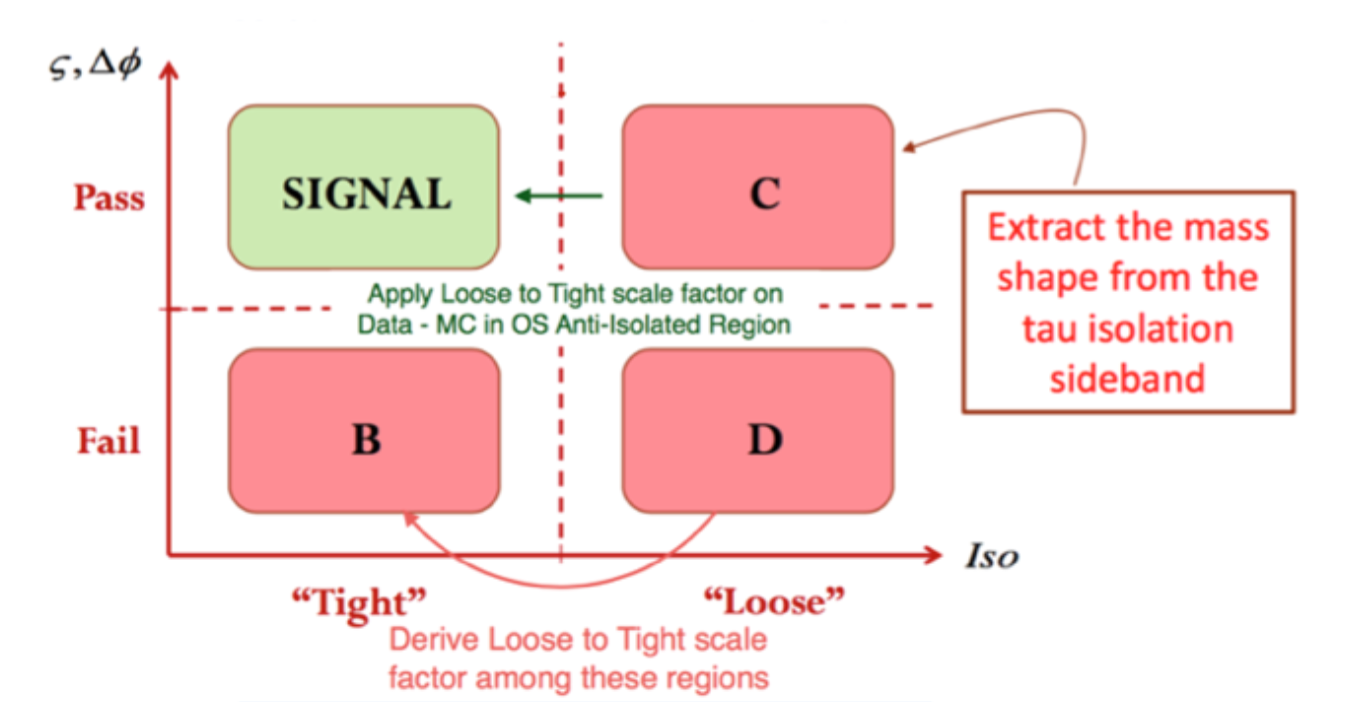
\includegraphics[width=0.5\textwidth]{figures/ABCD_muTau.png}
\caption{The four regions used in the ``ABCD" method of estimating W+Jets background}
\end{figure}

We estimate the W + Jets component $N_{W}^{i}$ in regions $i=A,B,C$ by subtracting MC non-W backgrounds
from data ($N_{W}^{i}=N_{\textrm{Data}}^{i}-N_{\neq W}^{i}$). We then estimate the W + Jets component in the signal region A, to
be $N_{W}^{A} = N_{W}^{C} \cdot \frac{N_{W}^{B}}{N_{W}^{D}}$. Said differently, we take the yield of W + Jets events in data containing a non-isolated $\tau_{h}$ 
and then extrapolate to the signal region by correcting for the ``Tight-to-Loose" ratio (also referred to as a ``fake rate"), which is measured in a data sample 
enriched with W + Jets events and that is obtained by inverting the $\zeta$ and cos$\Delta\phi$ cuts. The shape of the $m(\mu,\tau_{h},\MET)$ distribution is 
obtained from control region C (nominal selections with non-isolated $\tau_{h}$).

Figure~\ref{fig:ZetaAndCosDphiVsTauIso} shows a comparison of the $\zeta$ and cos$\Delta\phi$ distributions in W + Jets MC, normalized to unity, under two 
different $\tau_{h}$ isolation conditions: ($i$) isolated (passing ``"Tight"), and ($ii$) non-isolated (failing ``Tight" but passing loosened isolation). The 
$\tau_{h}$ isolation does not bias the $\zeta$ and cos$\Delta\phi$ distributions, and thus we expect our ABCD background estimation method to nicely model the ``true" W + 
jets yield in the signal region. A closure test for the background estimation method outlined above is performed with MC. Two aspects are simultaneously tested: 
(1) closure on the normalization (i.e. $N_{W}^{A} = N_{W}^{C} \cdot \frac{N_{W}^{B}}{N_{W}^{D}}$); (2) correct determination of the $m(\mu,\tau_{h},\MET)$ shape. 
Figure~\ref{fig:wJetsClosureMuTau} shows the closure test in MC. The y-axis of the top left plot is in normal scale so the reader can focus on the level of 
agreement in the low mass region. The top right plot is similar, except the y-axis is in log scale in order to emphasize the high-mass tails. We observe very 
good agreement between the nominal yield/shape and the predicted yield/shape. The reader can perform his or her own cross-check of this conclusion by using the 
MC-based W + Jets yields in Table \ref{tab:muTauWJetsCR}, which shows the data and MC background yields in the control samples, and plugging them into the 
equation $N_{W}^{\textrm{Prediction},MC} = N_{W}^{C,MC} \cdot \frac{N_{W}^{B,MC}}{N_{W}^{D,MC}}$. The MC-based prediction using the ABCD method is 
%$N_{W}^{\textrm{Prediction},MC} = (2222.81 \pm 75.60) \cdot \frac{(10443.71 \pm 163.29)}{(16046.17 \pm 201.87)} = 1446.68 \pm 57.13$, while the MC-based nominal 
%yield is $1510.98 \pm 62.85$ (see Table~\ref{tab:muTauCutFlowEff}). Therefore, the MC-based nominal yield to predicted yield ratio is 
%$\frac{N_{W}^{\textrm{Nominal},MC}}{N_{W}^{\textrm{Prediction},MC}} = \frac{1510.98 \pm 62.85}{1446.68 \pm 57.13} = 1.05 \pm 0.06$, which is statistically 
%consistent with unity. 
$N_{W}^{\textrm{Prediction},MC} = (1112.1 \pm 53.7) \cdot \frac{(5235.7 \pm 115.6)}{(7591.9 \pm 139.2)} = 766.9 \pm 43.1$, while the MC-based nominal 
yield is $757.9 \pm 35.0$ (see Table~\ref{tab:muTauCutFlowEff}). Therefore, the MC-based nominal yield to predicted yield ratio is 
$\frac{N_{W}^{\textrm{Nominal},MC}}{N_{W}^{\textrm{Prediction},MC}} = \frac{757.9 \pm 35.0}{766.9 \pm 43.1} = 0.99 \pm 0.05$, which is statistically 
consistent with unity. 
Thus, no additional systematic uncertainties are applied due to closure.

\begin{figure}\centering
  \includegraphics[width=0.4\textwidth]{figures/mt/WJetsClosure_Zeta1D_IsoVsNonIso_2p11ifb.png}
  \includegraphics[width=0.4\textwidth]{figures/mt/WJetsClosure_CosDphi_IsoVsNonIso_2p11ifb.png}
  \caption{\label{fig:ZetaAndCosDphiVsTauIso} Left: Comparison of the $\zeta$ distribution in W + Jets MC, normalized to unity, for events with isolated and 
non-isolated $\tau_{h}$.  Right: Comparison of the cos$\Delta\phi$ distribution in W + Jets MC, normalized to unity, for events with isolated and
non-isolated $\tau_{h}$.}
\end{figure}

\begin{figure}\centering
%  \includegraphics[width=0.4\textwidth]{figures/mt/WJetsClosure_NormalScale_2p11ifb.png}
%  \includegraphics[width=0.4\textwidth]{figures/mt/WJetsClosure_LogScale_2p11ifb.png} \\
  \includegraphics[width=0.4\textwidth]{figures/mt/WJetsClosure_NormalScale_2p11ifb_TightTo5WJetsIsoSideband.png}
  \includegraphics[width=0.4\textwidth]{figures/mt/WJetsClosure_LogScale_2p11ifb_TightTo5WJetsIsoSideband.png} \\
  \includegraphics[width=0.4\textwidth]{figures/mt/WJetsClosure_ForZtautauCR_NormalScale_2p11ifb.png}
  \includegraphics[width=0.4\textwidth]{figures/mt/WJetsClosure_ForZtautauCR_LogScale_2p11ifb.png} \\
  \includegraphics[width=0.4\textwidth]{figures/mt/WJetsClosure_NormalScale_2p11ifb_RegionA_vs_RegionB_ForIvan.png}
  \includegraphics[width=0.4\textwidth]{figures/mt/WJetsClosure_LogScale_2p11ifb_RegionA_vs_RegionB_ForIvan.png}
  \caption{\label{fig:wJetsClosureMuTau} Top Left: W + Jets closure test performed with simulation (normal scale to focus on low mass) under nominal $\MET$ 
conditions (i.e. $\MET > 30$ GeV).  Top Right: 
W + Jets closure test performed with simulation (log scale to focus on the high mass tails) under nominal $\MET$
conditions (i.e. $\MET > 30$ GeV).  Middle Left: W + Jets closure test performed 
with simulation (normal scale to focus on low mass), requiring $\MET > 0$ GeV.  Middle Right: W + Jets closure test performed with simulation (log scale to 
focus on the high mass tails), requiring $\MET > 0$ GeV.  Bottom Left: Comparison of the reconstructed mass distributions in regions A and B, in normal scale.  
Bottom Right: Comparison of the reconstructed mass distributions in regions A and B, in log scale.} 
\end{figure}

\begin{table}[htbp!]
  \centering{
  \caption{Background and data yields in W + Jets control regions $A,B,C$, under nominal $\MET$ conditions (i.e. $\MET > 30$ GeV).}  \label{tab:muTauWJetsCR}
    \begin{tabular}{| l | c | c | c | c |}
      \hline\hline
      Process & $\mu\tau_{h}$ W + Jets CR $B$ & $\mu\tau_{h}$ W + Jets CR $A$ & $\mu\tau_{h}$ W + Jets CR $C$ \\ [0.5ex] \hline
%      ZZ + Jets & 10.02 $\pm$ 3.22 & 7.15 $\pm$ 2.72 & 1.19 $\pm$ 1.11 \\
%      WZ + Jets & 35.93 $\pm$ 6.29 & 33.09 $\pm$ 6.04 & 3.29 $\pm$ 1.90 \\
%      WW + Jets & 186.09 $\pm$ 15.21 & 144.75 $\pm$ 13.42 & 24.75 $\pm$ 5.55 \\
%      QCD & 306.73 $\pm$ 122.65 & 793.18 $\pm$ 198.29 & 367.99 $\pm$ 135.06 \\
%      $t\bar{t}$ & 354.65 $\pm$ 20.23 & 352.76 $\pm$ 20.18 & 38.93 $\pm$ 6.70 \\
%      Z + Jets & 1899.95 $\pm$ 87.51 & 1579.47 $\pm$ 60.99 & 678.28 $\pm$ 55.34 \\
%      W + Jets & 10443.71 $\pm$ 163.29 & 16046.17 $\pm$ 201.87 & 2222.81 $\pm$ 75.60 \\
%      Data & 15546 & 21519 & 3501 \\
      ZZ + Jets & 8.5 $\pm$ 3.0 & 4.2 $\pm$ 2.1 & 0.7 $\pm$ 0.9 \\ 
      WZ + Jets & 24.4 $\pm$ 5.2 & 18.2 $\pm$ 4.5 & 1.8 $\pm$ 1.4 \\ 
      WW + Jets & 141.2 $\pm$ 13.3 & 86.2 $\pm$ 10.4 & 17.2 $\pm$ 4.6 \\ 
      QCD & 188.5 $\pm$ 96.2 & 631.3 $\pm$ 176.9 & 140.5 $\pm$ 83.4 \\ 
      $t\bar{t}$ & 249.6 $\pm$ 17.0 & 189.7 $\pm$ 14.8 & 22.8 $\pm$ 5.1 \\ 
      Z + Jets & 1278.2 $\pm$ 71.0 & 871.0 $\pm$ 46.5 & 425.7 $\pm$ 40.2 \\ 
      W + Jets & 5235.7 $\pm$ 115.6 & 7591.9 $\pm$ 139.2 & 1112.1 $\pm$ 53.7 \\ 
      Data & 8278 & 10434 & 1847 \\ 
      \hline
%      Purity & 78.90\% & 84.65\% & 66.61\% \\
      Purity & 73.5\% & 80.8\% & 64.6\% \\
%      Data - $\sum\limits_{i\neq W} BG_{i}$ & 12752.65 $\pm$ 278.56 & 18608.60 $\pm$ 312.88 & 2386.58 $\pm$ 175.68 \\
      Data - $\sum\limits_{i\neq W} BG_{i}$ & 6387.6 $\pm$ 201.5 & 8633.4 $\pm$ 237.2 & 1238.3 $\pm$ 111.8 \\
      \hline
%      SF & 1.22 $\pm$ 0.03 & 1.16 $\pm$ 0.02 & 1.07 $\pm$ 0.09 \\
      SF & 1.22 $\pm$ 0.05 & 1.14 $\pm$ 0.04 & 1.11 $\pm$ 0.11 \\ 
      \hline\hline
    \end{tabular}
  }
\end{table}

As mentioned above, Table \ref{tab:muTauWJetsCR} shows the data and MC background yields in control regions $A$, $B$, and $C$. The purity of W + Jets, based on 
simulation, ranges from $\sim 65-81$\%, depending on the sample. The W + Jets scale factors, defined as SF$=\frac{N^{\textrm{Data}}-N_{\neq 
W}^{MC}}{N_{W}^{MC}}$, show about a $\sim 20$\% mismodeling in simulation. The top row of plots in Figure~\ref{fig:wJetsControlPlotsMuTau} are the 
$m_{T}(\mu,\MET)$ distributions in control regions $C$(top left) and $A$(top right). The previously mentioned scale factors have been applied to the plots. 

A natural comment or question from the reader is that while the MC closure test looks good, it is possible that mis-modeled $\MET$ in simulation could perhaps 
pull the closure test in the wrong direction. In other words, how stable is the background estimation method with respect to $\MET$. The middle row of plots in 
Figure~\ref{fig:wJetsClosureMuTau} show similar closure tests, but without a $\MET$ cut. We find that closure is observed even without the $\MET$ cut, adding 
to the robustness of the methodology. Table \ref{tab:muTauWJetsCR_noMet} shows the data and MC background yields in control regions $A$, $B$, and $C$ obtained 
without the $\MET$ requirement. The purity 
of W + Jets, based on simulation, has decreased in comparison to the purity observed with $\MET > 30$ GeV, due to the larger contribution from DY + Jets and QCD 
multijet. 
%The W + Jets scale factors, similarly defined as SF$=\frac{N^{\textrm{Data}}-N_{\neq W}^{MC}}{N_{W}^{MC}}$, show consistency with unity. 
%Therefore, the $\sim 20$\% disagreement (SF$\sim 1.2$) observed in the control regions with nominal $\MET$ can be attributed to a mis-modeled $\MET$ cut 
%efficiency in simulation. 

\begin{figure}\centering
  \includegraphics[width=0.4\textwidth]{figures/mt/Muon1Tau1_Muon1MetMt_SRexceptNonIsolatedTau_25ns_2110ipb_VeryNonIsolatedTau_WjetsSF1p14.png}
  \includegraphics[width=0.4\textwidth]{figures/mt/Muon2Tau1_Muon2MetMt_SRexceptNonIsolatedTauexceptInvertedCosDphiexceptInvertedZeta_25ns_2110ipb_VeryNonIsolatedTau_WjetsSF1p14.png} \\
  \includegraphics[width=0.4\textwidth]{figures/mt/Muon1Tau1_Tau1MetDeltaPhi_SRexceptNonIsolatedTauexceptMet_25ns_2110ipb_VeryNonIsolatedTau_WjetsSF1p22.png}
  \includegraphics[width=0.4\textwidth]{figures/mt/Muon2Tau1_Tau1MetDeltaPhi_SRexceptNonIsolatedTauexceptMetexceptInvertedCosDphiexceptInvertedZeta_25ns_2110ipb_VeryNonisolatedTau_WjetsSF1p22.png}
  \caption{\label{fig:wJetsControlPlotsMuTau} Top Left: $m_{T}(\mu,\MET)$ distributions in W + Jets control region $C$, under nominal $\MET$
conditions (i.e. $\MET > 30$ GeV).  Top Right: $m_{T}(\mu,\MET)$ distributions in W + Jets control region $A$, under nominal $\MET$
conditions (i.e. $\MET > 30$ GeV).  Bottom Left:  $m_{T}(\mu,\MET)$ distributions in W + Jets control region $C$, requiring $\MET > 0$ GeV.  Bottom Right: 
$m_{T}(\mu,\MET)$ distributions in W + Jets control region $A$, requiring $\MET > 0$ GeV.} 
\end{figure}

\begin{table}[htbp!]
  \centering{
  \caption{Background and data yields in W + Jets control regions $A,B,C$ obtained without a $\MET$ requirement.}  \label{tab:muTauWJetsCR_noMet}
    \begin{tabular}{| l | c | c | c | c |}
      \hline\hline
      Process & $\mu\tau_{h}$ W + Jets CR $B$ & $\mu\tau_{h}$ W + Jets CR $A$ & $\mu\tau_{h}$ W + Jets CR $C$ \\ [0.5ex] \hline
%      ZZ + Jets & 16.18 $\pm$ 4.07 & 13.35 $\pm$ 3.70 & 2.37 $\pm$ 1.56 \\
%      WZ + Jets & 43.26 $\pm$ 6.82 & 41.23 $\pm$ 6.66 & 5.80 $\pm$ 2.50 \\
%      WW + Jets & 197.24 $\pm$ 15.27 & 162.60 $\pm$ 13.86 & 35.69 $\pm$ 6.50 \\
%      $t\bar{t}$ & 339.45 $\pm$ 19.46 & 340.78 $\pm$ 19.50 & 42.12 $\pm$ 6.85 \\
%      QCD & 3896.33 $\pm$ 379.20 & 4013.60 $\pm$ 385.02 & 2365.52 $\pm$ 295.58 \\
%      Z + Jets & 4190.96 $\pm$ 92.55 & 4573.54 $\pm$ 96.64 & 2256.33 $\pm$ 67.85 \\
%      W + Jets & 12233.43 $\pm$ 169.20 & 18688.29 $\pm$ 209.12 & 4483.98 $\pm$ 102.44 \\
%      Data & 25861 & 35560 & 11144 \\
      ZZ + Jets & 16.0 $\pm$ 4.1 & 9.6 $\pm$ 3.2 & 1.8 $\pm$ 1.4 \\
      WZ + Jets & 37.4 $\pm$ 6.4 & 26.2 $\pm$ 5.4 & 4.0 $\pm$ 2.1 \\ 
      WW + Jets & 183.6 $\pm$ 15.1 & 114.3 $\pm$ 11.9 & 29.0 $\pm$ 6.0 \\
      $t\bar{t}$ & 284.3 $\pm$ 18.1 & 222.6 $\pm$ 16.0 & 29.7 $\pm$ 5.9 \\
      QCD & 411.6 $\pm$ 141.9 & 1002.9 $\pm$ 221.7 & 442.1 $\pm$ 147.2 \\ 
      Z + Jets & 3282.9 $\pm$ 101.2 & 2754.5 $\pm$ 84.5 & 1870.1 $\pm$ 83.6 \\ 
      W + Jets & 7586.9 $\pm$ 139.3 & 10894.9 $\pm$ 166.7 & 2699.9 $\pm$ 84.6 \\ 
      Data & 13896 & 17235 & 5984 \\ 
      \hline
%      Purity & 58.49\% & 67.14\% & 48.78\% \\
      Purity & 64.28\% & 72.51\% & 53.18\% \\
%      Data - $\sum\limits_{i\neq W} BG_{i}$ & 11631.58 $\pm$ 708.78 & 18979.90 $\pm$ 747.02 & 4562.17 $\pm$ 456.33 \\
      Data - $\sum\limits_{i\neq W} BG_{i}$ & 9680.10 $\pm$ 394.34 & 13104.88 $\pm$ 400.66 & 3607.34 $\pm$ 267.70 \\
      \hline
%      SF & 0.95 $\pm$ 0.06 & 1.02 $\pm$ 0.04 & 1.02 $\pm$ 0.10 \\
      SF & 1.28 $\pm$ 0.06 & 1.20 $\pm$ 0.04 & 1.34 $\pm$ 0.11 \\
      \hline\hline
    \end{tabular}
  }
\end{table}

The procedure outlined in this section yields a W + Jets estimate of $N_{W}^{\textrm{Prediction,Data}} = (1238.3 \pm 111.8) \cdot \frac{(6387.6 
\pm 201.5)}{(8633.4 \pm 237.2)} = 916.2 \pm 91.2$ (see Data - $\sum\limits_{i\neq W} BG_{i}$ in Table \ref{tab:muTauWJetsCR}). The uncertainty on the 
background prediction is $\sim 10$\% and is mostly dominated by $\sqrt{N_{\textrm{Data}}}$ in control regions $A$, $B$, and $C$. We note that the main source of 
contamination in Table \ref{tab:muTauWJetsCR} is DY + Jets, which we've normalized using a data-to-MC correction factor described in the next section. However, 
even if DY + Jet(s) yields in the W control samples are taken entirely from simulation, it only provides a small effect on the W + Jets prediction in the signal region. This is true 
because the systematic uncertainty for DY + Jets is typically $< 15$\% (see section 10), while the level of non-W background contamination is at most $\sim 35$\% 
(i.e. upper bound on systematic effect is $0.35 \cdot 0.15 \sim 5$\%). The total predicted background
$m(\mu,\tau_{h},\MET)$ spectrum will be shown in the results section of this chapter.

\subsubsection{W + Jets Background Validation with High mT}

The standard approach to estimate the W + Jets background in the Higgs search is to use a control sample of events with high $m_{T}(\mu,\MET)$. 
The W + Jets yield in that region is determined by subtracting the non-W predictions from data using simulation, and subsequently extrapolating to the 
signal region using an extrapolation factor determined from MC. We do not employ a similar approach in this analysis as we are motivated by wanting a fully 
data-driven approach to estimating both the normalization and the mass shape. However, we use a similar control sample of high $m_{T}(\mu,\MET)$ events to 
validate our background estimation method and provide further confidence in our method. For this purpose we select events with $m_{T}(\mu,\MET) > 70$ GeV in 
addition to the signal region selections. The MC-based W + Jets yield in this high $m_{T}(\mu,\MET)$ control sample is corrected using a scale factor equal to the 
ratio of the data-driven and nominal W + Jets yields in the signal region. Table~\ref{tab:muTauHighMt} shows the data and background yields in this high 
$m_{T}(\mu,\MET)$ control sample, while Figure~\ref{fig:muTauHighMtControlPlots} shows the $p_{T}(\tau_{h})$ and $\eta(\tau_{h})$ distributions. The measured 
scale factor, $0.90 \pm 0.11$, is consistent with unity and therefore provides further validation of our background estimation methodology.

\begin{table}[htbp!] 
\begin{center}
 \caption{ Events in the W + Jets high $m_{T}(\mu,\MET)$ control region for data and MC.}
 \begin{tabular}{| l | c |}
 \hline\hline
Data & 731 \\
W + Jets & 580.2 $\pm$ 39.5 \\
Z + Jets & 135.9 $\pm$ 17.0 \\
WZ + Jets & 2.9 $\pm$ 1.8 \\
WW + Jets & 15.3 $\pm$ 4.4 \\
ZZ + Jets & 0.2 $\pm$ 0.5 \\
QCD & 36.1 $\pm$ 39.4 \\
$t\bar{t}$ & 17.7 $\pm$ 4.5 \\ \hline
Purity & 73.6\% \\
Data - $\sum\limits_{i} BG_{i}$ & 522.9 $\pm$ 51.1 \\ \hline
SF & 0.9 $\pm$ 0.1 \\
 \hline
 \hline
 \end{tabular}
 \label{tab:muTauHighMt}
\end{center}
\end{table}

\begin{figure}[thbp!]\centering 
  \includegraphics[width=0.4\textwidth]{figures/mt/ControlPlots_FirstLeadingTauJet1Pt_AfterFinalselectionsWithHighMt.png}
  \includegraphics[width=0.4\textwidth]{figures/mt/ControlPlots_FirstLeadingTauJet1Eta_AfterFinalselectionsWithHighMt.png} 
  \caption{\label{fig:muTauHighMtControlPlots} Event yields vs $p_{T}(\tau_{h})$ and $\eta(\tau_{h})$ in the W + Jets high $m_{T}(\mu,\MET)$ control region.}
\end{figure}

\subsection{DY + Jets Background Estimation}

Obtaining a semi-clean sample of $Z\to\tau\tau$ events is one of the most important aspects of the analysis as it needs to be shown the $\tau_{h}$ identification 
criteria employed is successful at identifying a $\tau_{h}$. Unlike W + Jets, where a jet is misidentified as a $\tau_{h}$ and whose contribution to the 
signal region is expected to be mismodeled by simulation, there is no reason to expect significant disagreement between data and MC for $Z\to\tau\tau$. The 
efficiency for the requirement of a high quality muon and $\tau_{h}$ candidate is expected to be well modeled by simulation, and has indeed been validated by the 
POGs. Moreover, the $\MET$ in $Z\to\tau\tau$ events is ``real" missing momentum from the escaping neutrinos produced by the $\tau$-lepton decay, 
and thus is also expected to be well modeled by simulation. Therefore, the estimate of the DY + Jets contribution ($\sim 98$\% $Z\to\tau\tau$) is based on both 
simulation and data. We utilize a scale factor, defined as the ratio of efficiencies measured in data and simulation, to normalize the predicted rate 
to the data by correcting the expected DY + Jets contribution obtained from MC. A semi-clean sample of $Z \to \tau\tau$ events is obtained with the following 
modifications to the final signal selections:
%Therefore, obtaining a semi-clean sample of $Z \to \tau\tau$ events where the number of 
%observed events are consistent with the MC expectation ensures the robustness of the analysis and validates the ability to successfully identify taus. A 
%data-driven measurement of the $Z\rightarrow\tau\tau$ contribution in the signal region is not employed. Instead, an MC based approach is employed to show that 
%data and MC are consistent in the control region. To validate the MC predictions, the following modifications are made to the final signal selections:

\begin{itemize}
\item $\MET < 30$ GeV 
\item $m(\mu,\tau_{h},\MET) < 300$ GeV
\end{itemize}

It is important to note that the analysis has been designed to achieve sensitivity in the high mass region, while also enabling us to achieve a relatively clean 
$Z\rightarrow\tau\tau$ signature in the low mass region with only minor modifications to the final selections. Figure~\ref{fig:ZtautauControlPlots} shows the 
$m(\mu,\tau_{h},\MET)$ invariant mass in the $Z\rightarrow\tau\tau$ control region defined above, while the observed events in data and predicted 
background yields are listed in Table~\ref{table:theztautauControlTable} (W + Jets and QCD multijet backgrounds are completely data-driven).

\begin{table}[htbp!]
\begin{center}
 \caption{ Events in the $Z\rightarrow\tau\tau$ control region for data and MC.}
 \begin{tabular}{| l | c |}
 \hline\hline
%Process & $\MET < 30$ GeV, $m(\mu,\tau_{h},\MET) < 300$ GeV \\ \hline
%Data & 10164 \\
%W + Jets & 5058.57 $\pm$ 235.401 \\
%Z + Jets & 4460.44 $\pm$ 110.06 \\
%WZ + Jets & 12.1583 $\pm$ 3.6595 \\
%WW + Jets & 64.3483 $\pm$ 8.946 \\
%ZZ + Jets & 3.74661 $\pm$ 1.96897 \\
%QCD & 365.39 $\pm$ 133.691 \\
%$t\bar{t}$ & 46.3425 $\pm$ 7.31457 \\ \hline
%%Purity & 44.5554\% \\
%Data - $\sum\limits_{i} BG_{i}$ & 4613.45 $\pm$ 289.14 \\ \hline
%SF & 1.0343 $\pm$ 0.069666 \\
Data & 6658 \\
W + Jets & 2586.9 $\pm$ 168.2 \\
Z + Jets & 3806.1 $\pm$ 100.7 \\
WZ + Jets & 9.0 $\pm$ 3.1 \\
WW + Jets & 48.8 $\pm$ 7.8 \\
ZZ + Jets & 2.8 $\pm$ 1.7 \\
QCD & 319.8 $\pm$ 125.1 \\
$t\bar{t}$ & 33.0 $\pm$ 6.2 \\ \hline
Purity & 55.9\% \\
Data - $\sum\limits_{i} BG_{i}$ & 3657.8 $\pm$ 225.2 \\ \hline
SF & 0.96 $\pm$ 0.06 \\
 \hline
 \hline
 \end{tabular}
 \label{table:theztautauControlTable}
\end{center}
\end{table}

\begin{figure}
\begin{center}
%\includegraphics[angle=0,width=.75\textwidth]{figures/mt/Muon1Tau1ReconstructableMass_SRexceptMet_WJetsDataDriven_25ns_2110ipb.png}
\includegraphics[angle=0,width=.75\textwidth]{figures/mt/Muon1Tau1ReconstructableMass_SRexceptMet_WJetsDataDriven_25ns_2110ipb_1or3prong.png}
\caption{ $m(\mu,\tau_{h},\MET)$ distribution in the $Z \to \tau\tau$ control region defined by $\MET < 30$ GeV and $m(\mu,\tau_{h},\MET) < 300$ GeV, with 
otherwise similar selections to the signal region. $Z \to \tau\tau$ (DY+Jets) events are shown in blue.}
\label{fig:ZtautauControlPlots}
\end{center}
\end{figure}

Table~\ref{table:theztautauControlTable} and Figure~\ref{fig:ZtautauControlPlots} clearly show that both the $Z \to \tau\tau$ rates and shapes are consistent 
between data and MC, with a SF approximately $0.96 \pm 0.06$. Therefore, the expected $Z \to \tau\tau$ contribution in the signal region is taken from MC. The 
expected number of $Z \to \tau\tau$ events in the signal region is $883 \pm 35$ (see Table~\ref{tab:muTauCutFlowEff}). 
Obtaining a semi-clean sample of $Z \to \tau\tau$ events where the number of observed events are consistent with the MC expectation ensures the robustness of the 
analysis and validates the ability to successfully identify a $\tau_{h}$. Furthermore, since our $\tau_{h}$ identification efficiency is ``flat" vs. 
$p_{T}(\tau_{h})$, validating correct modeling of $Z \to \tau\tau$ at low $p_{T}(\tau_{h})$ indirectly ``validates" that we can correctly identify a high-$p_{T}$ 
$\tau_{h}$. The total predicted background $m(\mu,\tau_{h},\MET)$ spectrum will be shown in the results section of the AN.

\subsection{Other Small Backgrounds}

As mentioned in the introduction to section~\ref{sec:muTauhad} and as can be calculated from Table~\ref{tab:muTauCutFlowEff}, the sum of the Drell-Yan and W + 
jets backgrounds represent approximately $93$\% of the total background in this channel. The remaining $t\bar{t}$, diboson, and QCD multijet processes compose 
$\sim$ 1.3\%, 1.4\%, and 4.4\% of the total background respectively. Therefore, these backgrounds are taken directly from simulation with appropriate systematic 
uncertainties, which are discussed and summarized in section 10. Furthermore, the $t\bar{t}$ and diboson backgrounds are expected to be well modeled by simulation 
and thus, for added confidence, we only perform a validation of the ``good enough" modeling of the QCD multijet background. For this purpose, we obtain a control 
sample enriched with $\sim 91$\% purity of QCD multijet events by inverting the isolation on both the $\tau_{h}$ and $\mu$ legs as well as inverting the 
$\mu\tau_{h}$ charge requirement (select like-sign). Table~\ref{table:theQCDMuTauControlTable} summarizes the observed data events and predicted background yields 
in this sample. The measured data-to-MC correction factor of $\textrm{SF}=1.09 \pm 0.27$ is consistent with unity, and thus the QCD multijet yields (in the 
signal and control regions) are taken directly from simulation. The QCD multijet contribution to the signal region is conservatively assigned an additional $27$\% 
systematic uncertainty based on the uncertainty on the correction factor from this control sample (this is on top of the $\sim 63$\% statistical uncertainty).

\begin{table}[htbp!]
\begin{center}
 \caption{ Yields in the $\mu\tau_{h}$ QCD control region for data and MC.}
 \begin{tabular}{| l | c |}
 \hline\hline
Process & non-isolated $\tau_{h}$, non-isolated $\mu$, same-sign $\mu\tau_{h}$ \\ \hline
Data & 442 \\
W + Jets & 33.1 $\pm$ 9.2 \\
Z + Jets & 1.4 $\pm$ 1.3 \\
WZ & 0.34 $\pm$ 0.61 \\
WW & 0 $\pm$ 0 \\
ZZ & 0 $\pm$ 0 \\
QCD & 371.6 $\pm$ 90.8 \\
$t\bar{t}$ & 1.7 $\pm$ 1.4 \\ \hline
Purity & 91.0\% \\
Data - $\sum\limits_{i} BG_{i}$ & 405.4 $\pm$ 23.0 \\ \hline
SF & 1.09 $\pm$ 0.27 \\
 \hline
 \hline
 \end{tabular}
 \label{table:theQCDMuTauControlTable}
\end{center}
\end{table}

